\section{Technical Overview}
A simplified overview of the da Vinci setup is provided in \autoref{fig:overview} as a block diagram. The setup is physically located at the department of Control and Automation at Aalborg University in the laboratory. The figure is structured with the highest abstraction layer at the top (i.e. the ROS (Robotic Operation System)) and the lowest in the bottom, i.e. the actuators in form of seven Maxon motors.

The focus of this thesis is the highest abstraction layer, i.e.the ROS environment.
\begin{figure}[H]
	\center
	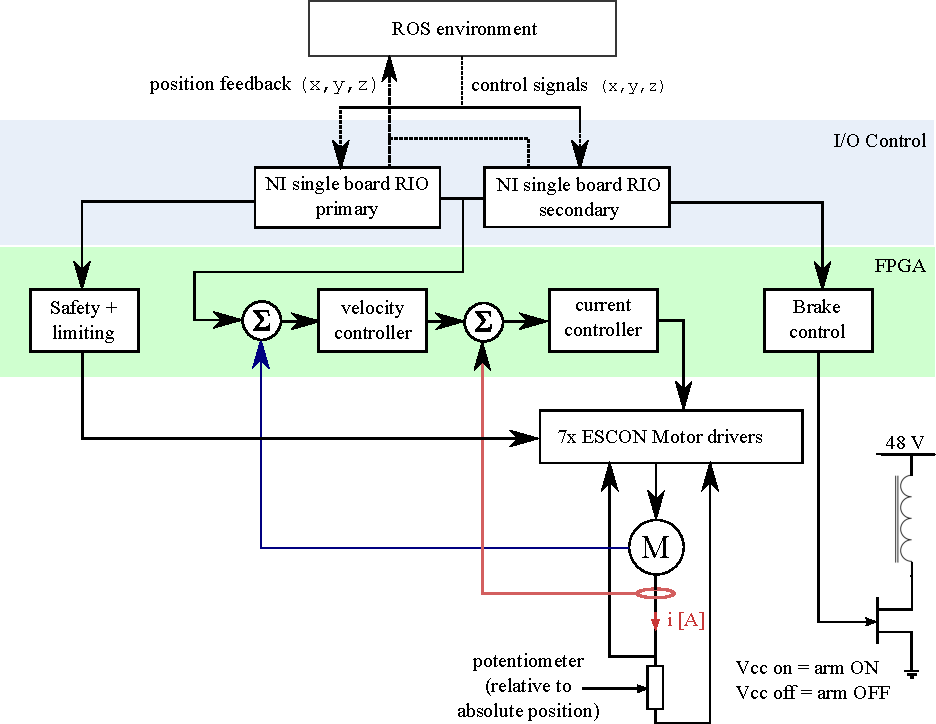
\includegraphics[width=0.95\textwidth]{overview.pdf}	\caption{This is a nice figure. Here illustrated for hand roll master.}
	\label{fig:overview}
\end{figure}

testing some stuff..
